\section{Proof of Theorem~\ref{thm:incompleteness}}
\label{sec:incompleteness}

We use the variant of the Cai--F\"urer--Immerman (CFI)
construction~\cite{CaiFurerImmerman1992} given
in~\cite[Definition~3.1]{Roberson2026}.
Let $B$ be a connected graph and $v_*$ a vertex of $B$.
For a vertex $v$ of $B$, the set of edges incident with $v$ is denoted by
$E_B(v)$.
For $i\in\{0,1\}$, let $\CFI_i(B)$ be the graph with
\begin{equation}\label{eq:ss-cfi-definition}
 \begin{aligned}
 \Xi_i(v)&=\left\{\xi\in\mathbb F_2^{E_B(v)}:
   \sum_{e\in E_B(v)}\xi_e=i\delta_{v,v_*}\right\},\\
 V(\CFI_i(B))&=\{(v,\xi):v\in V(B),\xi\in \Xi_i(v)\},\\
 E(\CFI_i(B))&=\{(v,\xi)(w,\zeta):vw\in E(B),\xi\in \Xi_i(v),\zeta\in \Xi_i(w),\xi_{vw}=\zeta_{vw}\}.
 \end{aligned}
\end{equation}
Here $\delta_{ab}$ is $1$ when $a=b$ and $0$ otherwise.
The vertices $(v,\xi)$ with $\xi\in \Xi_i(v)$ form a \emph{fibre} with
\emph{base vertex} $v$, and they are said to lie \emph{over} $v$.
The isomorphism type of $\CFI_1(B)$ is independent of the choice of
$v_*$, and the graphs $\CFI_0(B)$ and $\CFI_1(B)$ are non-isomorphic;
both facts follow from \cite[Lemma~5]{Neuen2024}.

For $i\in\{0,1\}$, let $\pi_i:\CFI_i(B)\to B$ be the projection
$\pi_i(v,\xi)=v$.
Let $F$ be a graph and $\chi:F\to B$ a homomorphism.
A homomorphism $f:F\to\CFI_i(B)$ is a \emph{lift} of $\chi$ if
$\pi_i\circ f=\chi$.
The number of such lifts is denoted by $\hom_\chi(F,\CFI_i(B))$.
We show that if $\hom(F,\CFI_0(B))=\hom(F,\CFI_1(B))$, then
$\hom_\chi(F,\CFI_0(B))=\hom_\chi(F,\CFI_1(B))$ for every homomorphism
$\chi:F\to B$.
For every fixed $\chi$, \cite[Theorem~3.6]{Roberson2026} gives
\begin{equation}\label{eq:ss-coloured-monotonicity}
  \hom_\chi(F,\CFI_1(B))\leq\hom_\chi(F,\CFI_0(B)).
\end{equation}
Every homomorphism $f:F\to\CFI_i(B)$ is a lift of exactly one map
$\chi=\pi_i\circ f$, so
\begin{equation}\label{eq:ss-lift-differences}
 \hom(F,\CFI_0(B))-\hom(F,\CFI_1(B))
 =\sum_\chi\bigl(\hom_\chi(F,\CFI_0(B))-\hom_\chi(F,\CFI_1(B))\bigr)
\end{equation}
is a sum of nonnegative terms. If the total counts agree, every term
therefore vanishes.
Consequently, for every graph $F$ and every homomorphism
$\chi:F\to B$,
\begin{equation}\label{eq:ss-lift-equality}
 \hom(F,\CFI_0(B))=\hom(F,\CFI_1(B))
 \Longrightarrow
 \hom_\chi(F,\CFI_0(B))=\hom_\chi(F,\CFI_1(B)).
\end{equation}

For a minor-closed class $\mathcal C$, the following lemma constructs
non-isomorphic graphs $G\equiv_{\mathcal C}G'$ with simple spectrum
whenever $\CFI_0(B)\equiv_{\mathcal C}\CFI_1(B)$.

\begin{lemma}\label{lem:ss-transfer}
Let $\mathcal C$ be a minor-closed graph class and let $B$ be a connected
graph satisfying $\CFI_0(B)\equiv_{\mathcal C}\CFI_1(B)$. Then there are non-isomorphic
graphs $G,G'$ with simple spectrum and $G\equiv_{\mathcal C}G'$.
The witnesses can be chosen bipartite, cospectral, nonsingular, and of
maximum degree at most six.
\end{lemma}

\begin{proof}[Proof of \cref{thm:incompleteness}]
By \cref{lem:ss-transfer}, it suffices to give, for each of the three
classes $\mathcal C$, a connected graph $B$ with
$\CFI_0(B)\equiv_{\mathcal C}\CFI_1(B)$.
When $\mathcal C$ is the class of graphs of treewidth at most $k\geq1$, the graph
$B=K_{k+2}$ satisfies
$\CFI_0(B)\equiv_{\mathcal C}\CFI_1(B)$~\cite[Theorem~10 and Lemma~12]{Neuen2024}.
When $\mathcal C$ is the class of graphs of Euler genus at most $g$, a connected
graph $B$ with $\CFI_0(B)\equiv_{\mathcal C}\CFI_1(B)$ is given in
\cite[Lemma~2.10 and proof of Theorem~1.8]{NeuenSeppelt2026}.
When $\mathcal C$ is the class of $K_7$-minor-free graphs, a connected graph $B$ with
$\CFI_0(B)\equiv_{\mathcal C}\CFI_1(B)$ is given in
\cite[Lemma~2.10 and proof of Theorem~1.9]{NeuenSeppelt2026}
and \cite[Theorem~1.7 and Section~1.3]{ThilikosWiederrecht2024}.
\end{proof}

The proof of \cref{lem:ss-transfer} has two steps.
If $\CFI_0(B)\equiv_{\mathcal C}\CFI_1(B)$ for a minor-closed class
$\mathcal C$, then the two graphs obtained from $\CFI_0(B)$ and
$\CFI_1(B)$ by attaching the same rooted graph to every vertex of a
fibre are again homomorphism indistinguishable over $\mathcal C$
(\cref{lem:ss-attachments}).
For a suitable choice of attached trees, the resulting graphs have
simple spectrum (\cref{lem:ss-cfi-spectrum}).
The second step uses two lemmas on the attached trees
(\cref{lem:ss-caterpillars,lem:ss-separation}).

Attaching a copy of a rooted graph at a vertex means identifying the
root of the copy with that vertex.
Fix a connected base graph $B$.
For each $z\in V(B)$, let $T_z$ be a rooted graph with root $r_z$.
Let the \emph{rooted product} $\widehat B$ be the graph obtained by
attaching one copy of $T_z$ at each $z\in V(B)$
and retaining all edges of $B$.
For $i\in\{0,1\}$, let the \emph{CFI-compatible rooted product}
$\widehat{\CFI}_i(B)$ be the graph obtained by attaching a separate copy
of $T_v$ at each $(v,\xi)\in V(\CFI_i(B))$ and retaining all edges of $\CFI_i(B)$.
In both products, each attached copy includes its root.
The projection $\pi_i$ extends to
$\widehat\pi_i:\widehat{\CFI}_i(B)\to\widehat B$ by mapping
each attached copy of $T_z$ identically onto the copy of $T_z$ in $\widehat B$.
\Cref{fig:ss-cfi-example} shows $B$, $\CFI_1(B)$ and their rooted
products for a base graph with three vertices.

\begin{figure}[tb]
\centering
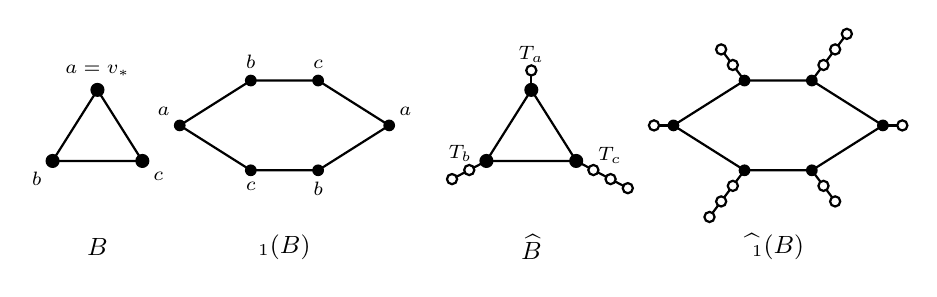
\begin{tikzpicture}[
  scale=.95,
  base/.style={circle,fill,inner sep=1.8pt},
  cfi/.style={circle,fill,inner sep=1.5pt},
  att/.style={circle,draw,fill=white,inner sep=1.3pt},
  lab/.style={font=\scriptsize,inner sep=1.5pt},
  line width=.8pt,
  every node/.style={font=\small},
]
\def\treeA#1#2{\draw (#1)--++(#2:.26) node[att]{};}
\def\treeB#1#2{\draw (#1)--++(#2:.26) node[att]{}--++(#2:.26) node[att]{};}
\def\treeC#1#2{\draw (#1)--++(#2:.26) node[att]{}--++(#2:.26) node[att]{}
                --++(#2:.26) node[att]{};}
\pgfmathsetmacro{\baseAngle}{atan2(.95/3,.6)}
\pgfmathsetmacro{\cfiAngle}{atan2(.6,.45)}
\foreach \attached in {0,1} {
  \begin{scope}[xshift={5.8*\attached cm}]
    \coordinate (a) at (0,.55);
    \coordinate (b) at (-.6,-.4);
    \coordinate (c) at (.6,-.4);
    \draw (a)--(b)--(c)--cycle;
    \ifnum\attached=0
      \node[base,label={[lab]above:$a=v_*$}] at (a) {};
      \node[base,label={[lab]below left:$b$}] at (b) {};
      \node[base,label={[lab]below right:$c$}] at (c) {};
      \node at (0,-1.55) {$B$};
    \else
      \treeA{a}{90}
      \treeB{b}{180+\baseAngle}
      \treeC{c}{360-\baseAngle}
      \node[lab,above] at (0,.85) {$T_a$};
      \node[lab,above] at (-.95,-.48) {$T_b$};
      \node[lab,above] at (1.05,-.5) {$T_c$};
      \foreach \v in {a,b,c} \node[base] at (\v) {};
      \node at (0,-1.55) {$\widehat B$};
    \fi
    \begin{scope}[xshift={(2.5+.8*\attached)*1cm}]
      \coordinate (a0) at (-1.4,.075);
      \coordinate (b0) at (-.45,.675);
      \coordinate (c0) at (.45,.675);
      \coordinate (a1) at (1.4,.075);
      \coordinate (b1) at (.45,-.525);
      \coordinate (c1) at (-.45,-.525);
      \draw (a0)--(b0)--(c0)--(a1)--(b1)--(c1)--cycle;
      \ifnum\attached=0
        \node[cfi,label={[lab]above left:$a$}] at (a0) {};
        \node[cfi,label={[lab]above:$b$}] at (b0) {};
        \node[cfi,label={[lab]above:$c$}] at (c0) {};
        \node[cfi,label={[lab]above right:$a$}] at (a1) {};
        \node[cfi,label={[lab]below:$b$}] at (b1) {};
        \node[cfi,label={[lab]below:$c$}] at (c1) {};
        \node at (0,-1.55) {$\CFI_1(B)$};
      \else
        \treeA{a0}{180} \treeA{a1}{0}
        \treeB{b0}{180-\cfiAngle} \treeB{b1}{360-\cfiAngle}
        \treeC{c0}{\cfiAngle}     \treeC{c1}{180+\cfiAngle}
        \foreach \v in {a0,b0,c0,a1,b1,c1} \node[cfi] at (\v) {};
        \node at (0,-1.55) {$\widehat{\CFI}_1(B)$};
      \fi
    \end{scope}
  \end{scope}
}
\end{tikzpicture}
\caption{A CFI-compatible rooted product for $B=K_3$ with $v_*=a$.
The hexagon labels indicate the base vertices of the fibres.
The attached paths $T_a,T_b,T_c$ have lengths one, two and three;
each vertex in the fibre over $z$ receives a copy of $T_z$.}
\label{fig:ss-cfi-example}
\end{figure}


\begin{lemma}\label{lem:ss-attachments}
Let $\mathcal C$ be a minor-closed graph class and $B$ a connected graph
such that $\CFI_0(B)\equiv_{\mathcal C}\CFI_1(B)$.
For any family of rooted graphs $(T_z)_{z\in V(B)}$, the CFI-compatible
rooted products satisfy
$\widehat{\CFI}_0(B)\equiv_{\mathcal C}\widehat{\CFI}_1(B)$.
\end{lemma}
\begin{proof}
Fix $F\in\mathcal C$.
We prove that, for $i\in\{0,1\}$,
\begin{equation}\label{eq:ss-attachment-count}
 \hom(F,\widehat{\CFI}_i(B))=
 \sum_{\eta:F\to\widehat B}\hom_{\chi_\eta}(Q_\eta,\CFI_i(B)),
\end{equation}
where, for each homomorphism $\eta:F\to\widehat B$, the graph $Q_\eta$
and the homomorphism $\chi_\eta:Q_\eta\to B$ are defined below.
The graph $Q_\eta$ is obtained from $F$ by contracting the connected
components of a subgraph of $F$ and replacing parallel edges by single edges, so
$Q_\eta$ is a minor of $F$, hence $Q_\eta\in\mathcal C$ because
$\mathcal C$ is minor-closed.
Since $\CFI_0(B)\equiv_{\mathcal C}\CFI_1(B)$ and $Q_\eta\in\mathcal C$,
we have $\hom(Q_\eta,\CFI_0(B))=\hom(Q_\eta,\CFI_1(B))$.
By \cref{eq:ss-lift-equality},
$\hom_{\chi_\eta}(Q_\eta,\CFI_0(B))=\hom_{\chi_\eta}(Q_\eta,\CFI_1(B))$.
Assuming \cref{eq:ss-attachment-count}, summing these equalities over $\eta$
gives $\hom(F,\widehat{\CFI}_0(B))=\hom(F,\widehat{\CFI}_1(B))$, which
proves the lemma.
It remains to define $Q_\eta$ and $\chi_\eta$ and to prove
\cref{eq:ss-attachment-count}.

For each homomorphism $\eta:F\to\widehat B$, define the following graphs and map.
Define a subgraph $F_\eta$ of $F$
with vertex set $V(F)$ by retaining an edge $vw\in E(F)$ if and only if
$\eta$ maps $vw$ to an edge of one of the attached copies $T_z$ in $\widehat B$.
Let $Q_\eta$ be the simple graph obtained from $F$ by contracting each
connected component of $F_\eta$ to one vertex and replacing parallel
edges by single edges; its vertices are the connected components of $F_\eta$.
Two distinct components are adjacent in $Q_\eta$ if and only if an edge of
$F$ has one endpoint in each component.
Every vertex of $\widehat B$ lies in exactly one attached copy, and the
edges of $F_\eta$ map into attached copies, so for each connected
component $K$ of $F_\eta$ there is a unique $z\in V(B)$ whose copy of
$T_z$ contains $\eta(K)$; we define $\chi_\eta(K)=z$.
If $vw\in E(F)$ has $v\in K$ and $w\in L$ for distinct components $K,L$, then
$\eta(v)\eta(w)$ is an edge of $B$ with endpoints $\chi_\eta(K)$ and
$\chi_\eta(L)$.
Hence $\chi_\eta:Q_\eta\to B$ is a homomorphism.

To prove \cref{eq:ss-attachment-count}, we fix $\eta$ and construct a
bijection between homomorphisms
$f:F\to\widehat{\CFI}_i(B)$ satisfying $\widehat\pi_i\circ f=\eta$
and lifts $h:Q_\eta\to\CFI_i(B)$ of $\chi_\eta$.
Given such an $f$, each connected component $K$ of $F_\eta$ maps
into a single attached copy, since every edge of $K$ projects into some
$T_z$. Let $h(K)$ be the root of this copy.
Then $\pi_i\circ h=\chi_\eta$, and edges between components map to edges
of $\CFI_i(B)$, so $h$ is a lift of $\chi_\eta$.

Conversely, let $h$ be a lift of $\chi_\eta$.
For each component $K$ of $F_\eta$, a copy of $T_{\chi_\eta(K)}$
is attached at $h(K)$ because $\pi_i(h(K))=\chi_\eta(K)$.
The projection $\widehat\pi_i$ maps this copy isomorphically onto
the copy of $T_{\chi_\eta(K)}$ in $\widehat B$.
For each $v\in K$, there is therefore a unique vertex $f(v)$ in the
copy rooted at $h(K)$ such that $\widehat\pi_i(f(v))=\eta(v)$.
Edges within a component are preserved by this isomorphism.
If $vw\in E(F)$ has $v\in K$ and $w\in L$ for distinct components $K,L$, then $\eta(v)$ and
$\eta(w)$ are roots. Hence $f(v)=h(K)$ and $f(w)=h(L)$, which are
adjacent because $h$ is a homomorphism.
The map $f\mapsto h$ and the map $h\mapsto f$ are inverse to each
other, which proves the bijection.
Summing over $\eta:F\to\widehat B$ proves \cref{eq:ss-attachment-count}.
\end{proof}

We next choose the attached graphs to obtain simple spectrum
(\cref{lem:ss-cfi-spectrum}).
A \emph{rooted subcubic caterpillar} is a tree obtained from a nonempty path
by attaching at most one new leaf to each path vertex and choosing an
endpoint of the path as the root. This path is called its \emph{spine}.
Thus the maximum degree is at most three and
the root degree is at most two; these bounds are used for the degree
bound in \cref{lem:ss-cfi-spectrum}.
The family $\mathcal T$ consists of the rooted subcubic caterpillars
obtained from $K_2$ rooted at an endpoint by zero or more applications
of the following two operations.
For a tree with root $r$, operation $X$ adds two new vertices $r',v$
and the edges $r'v,vr$, making $r'$ the new root.
Operation $Y$ adds a new root $r'$ and a new leaf $v$, with edges
$rr',r'v$ (\cref{fig:ss-operations}).

\begin{figure}[tb]
\centering
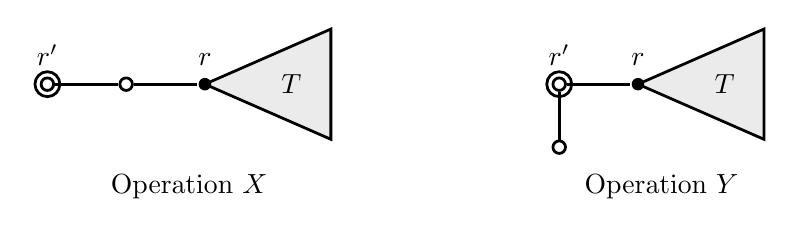
\begin{tikzpicture}[
  line width=1pt,
  old/.style={circle,fill,inner sep=1.6pt},
  new/.style={circle,draw,fill=white,inner sep=1.6pt},
  tree/.style={draw,fill=black!8},
]
\begin{scope}
  \draw[tree] (0,0) -- (1.6,0.7) -- (1.6,-0.7) -- cycle;
  \node at (1.1,0) {$T$};
  \node[old,label=above:$r$] (r) at (0,0) {};
  \node[new] (u) at (-1,0) {};
  \node[new,label=above:$r'$] (s) at (-2,0) {};
  \draw (s) -- (u) -- (r);
  \draw (s) circle (4.5pt);
  \node at (-0.2,-1.3) {Operation $X$};
\end{scope}
\begin{scope}[xshift=5.5cm]
  \draw[tree] (0,0) -- (1.6,0.7) -- (1.6,-0.7) -- cycle;
  \node at (1.1,0) {$T$};
  \node[old,label=above:$r$] (r) at (0,0) {};
  \node[new,label=above:$r'$] (s) at (-1,0) {};
  \node[new] (l) at (-1,-0.8) {};
  \draw (l) -- (s) -- (r);
  \draw (s) circle (4.5pt);
  \node at (0.3,-1.3) {Operation $Y$};
\end{scope}
\end{tikzpicture}
\caption{The operations $X$ and $Y$ applied to a rooted subcubic
caterpillar $T$ with root $r$. New vertices are white, and the new
root $r'$ is circled.}
\label{fig:ss-operations}
\end{figure}

We compute the characteristic polynomial of each $T\in\mathcal T$
recursively along its construction.
The adjacency matrix of a graph $H$ is denoted by $A_H$.
For the root $r$ of $T$, let $p_T(\lambda)=\det(\lambda I-A_T)$ and
$q_T(\lambda)=\det(\lambda I-A_{T-r})$ be the characteristic polynomials of $T$ and
$T-r$, respectively.
For a nonzero column $\xi=(p,q)^{\top}\in\R^2$, let
$[\xi]=[p:q]\in\mathbb P^1(\R)$ denote its span, identified with $p/q$ when $q\ne0$
and with $\infty$ when $q=0$.
In \cref{lem:ss-separation}, the eigenvalue multiplicities of the
rooted products depend on each attached tree $T$ only through the point
$h_T(\lambda)=[p_T(\lambda):q_T(\lambda)]$
(see \cref{lem:ss-rooted-multiplicity}).
We show that this point is defined for every real $\lambda$, that is,
$p_T(\lambda)$ and $q_T(\lambda)$ never vanish together.
The starting pair for rooted $K_2$ is
$(p_{K_2}(\lambda),q_{K_2}(\lambda))=(\lambda^2-1,\lambda)$.
By cofactor expansion, the operations $X$ and $Y$
transform the column $(p_T(\lambda),q_T(\lambda))^{\top}$ by multiplication
with the respective matrices
\begin{equation}\label{eq:ss-recurrence}
 \begin{aligned}
 \mathbf{X}_\lambda&=\begin{pmatrix}\lambda^2-1&-\lambda\\\lambda&-1\end{pmatrix},
 &\mathbf{Y}_\lambda&=\begin{pmatrix}\lambda^2-1&-\lambda\\\lambda&0\end{pmatrix}.
 \end{aligned}
\end{equation}
At $\lambda=0$, the recurrence \cref{eq:ss-recurrence} gives
$p_T(0)=(-1)^{|V(T)|/2}$ and $q_T(0)=0$.
These values are used for nonsingularity in \cref{lem:ss-separation}.
At $\lambda\ne0$, the starting pair is nonzero and both
matrices in \cref{eq:ss-recurrence} are invertible, so they carry
nonzero pairs to nonzero pairs.
Thus $h_T(\lambda)$ is defined for every real $\lambda$.

\begin{lemma}\label{lem:ss-caterpillars}
For any finite list of pairs
$(\lambda_j,a_j)\in\R^\times\times\mathbb P^1(\R)$, there is a tree
$T\in\mathcal T$ with $h_T(\lambda_j)\ne a_j$
for every $j$.
\end{lemma}
\begin{proof}
Let $\omega$ be a finite composition of the construction operations
$X,Y$, and let $T=\omega(K_2)$.
For each $j$, let $M_{\omega,j}$ be the matrix product obtained by
replacing each $X$ by $\mathbf{X}_{\lambda_j}$, each $Y$ by
$\mathbf{Y}_{\lambda_j}$, and composition by matrix multiplication.
For the empty composition, $M_{\omega,j}=I$.
Let $\nu_j=(p_{K_2}(\lambda_j),q_{K_2}(\lambda_j))^{\top}
=(\lambda_j^2-1,\lambda_j)^{\top}$.
Then $(p_T(\lambda_j),q_T(\lambda_j))^{\top}=M_{\omega,j}\nu_j$
by \cref{eq:ss-recurrence}.
Therefore, it suffices to find a composition $\omega$ such that
$[M_{\omega,j}\nu_j]\ne a_j$ for every $j$.

We express the conditions $[M_{\omega,j}\nu_j]\ne a_j$ for all $j$
as the nonvanishing of a linear functional on a tensor product.
For each $j$, define the linear functional
$\ell_j:\R^2\to\R$ by
\begin{equation}\label{eq:ss-avoidance-factors}
 \ell_j(p,q)=
 \begin{cases}
  p-a_jq,&a_j\in\R,\\
  q,&a_j=\infty.
 \end{cases}
\end{equation}
Let
$\nu=\bigotimes_j\nu_j$, $\ell=\bigotimes_j\ell_j$,
$\mathbf{X}=\bigotimes_j\mathbf{X}_{\lambda_j}$ and
$\mathbf{Y}=\bigotimes_j\mathbf{Y}_{\lambda_j}$,
where $\otimes$ is the tensor product.
Define $M_\omega$ in the same way using $\mathbf{X},\mathbf{Y}$.
Multiplication of tensor products gives
$M_\omega=\bigotimes_jM_{\omega,j}$.
Since $\ell$ is a tensor product of functionals,
\begin{equation}\label{eq:ss-positive-word}
 \ell(M_\omega\nu)=\prod_j\ell_j(M_{\omega,j}\nu_j),
\end{equation}
and each factor is nonzero exactly when
$h_T(\lambda_j)\ne a_j$.
Thus the avoidance conditions hold exactly when $\ell(M_\omega\nu)\ne0$.

It suffices to find a finite product $W$ of the matrices
$\mathbf{X}^{\pm1},\mathbf{Y}^{\pm1}$ with $\ell(W\nu)\ne0$.
Since every $\lambda_j\ne0$, the matrices $\mathbf{X},\mathbf{Y}$ are
invertible. By the Cayley--Hamilton theorem, their inverses are
polynomials in $\mathbf{X},\mathbf{Y}$, respectively.
Substituting these polynomial expressions into $W$ and expanding gives
a finite sum $W=\sum_i c_iM_{\omega_i}$, where $c_i\in\R$ and each
$\omega_i$ is a composition of the construction operations $X,Y$.
Consequently, $\ell(W\nu)=\sum_i c_i\ell(M_{\omega_i}\nu)\ne0$
implies $\ell(M_{\omega_i}\nu)\ne0$ for some $i$.
By \cref{eq:ss-positive-word}, the tree $T=\omega_i(K_2)$ then satisfies
$h_T(\lambda_j)\ne a_j$ for every $j$.

We now construct such a product $W$.
For $\lambda\ne0$, the matrices in \cref{eq:ss-recurrence} act on
$\mathbb P^1(\R)$ by multiplication of column representatives.
Let $D_\lambda=\mathbf{X}_\lambda^{-1}\mathbf{Y}_\lambda$.
On $\mathbb P^1(\R)$, $D_\lambda$ acts by
$t\mapsto\lambda^{-2}t+\lambda^{-1}$.
The starting value is $h_{K_2}(\lambda)=\lambda-\lambda^{-1}=\mathbf{Y}_\lambda\infty$.
Since $\mathbf{Y}_\lambda^{-1}\infty=0$, we have
$\mathbf{Y}_\lambda^{-2}h_{K_2}(\lambda)=0$.
Thus $D_\lambda^m\mathbf{Y}_\lambda^{-2}$ sends the starting value to
$\lambda^{-1}\sum_{k=0}^{m-1}\lambda^{-2k}$.
These values are strictly monotone in $m$ for every real $\lambda\ne0$,
so each $a_j$ is attained for at most one $m$ at $\lambda=\lambda_j$.
Choose a positive integer $m$ such that
$[D_{\lambda_j}^m\mathbf{Y}_{\lambda_j}^{-2}\nu_j]\ne a_j$ for every $j$.
Then $W=(\mathbf{X}^{-1}\mathbf{Y})^m\mathbf{Y}^{-2}$ satisfies
$\ell(W\nu)=\prod_j\ell_j(D_{\lambda_j}^m\mathbf{Y}_{\lambda_j}^{-2}\nu_j)\ne0$,
as required.
\end{proof}

For a base graph with edge weights, the rooted product retains the
original edge weights, and the edges of each $T_z$ have weight one.

\begin{lemma}\label{lem:ss-rooted-multiplicity}
Let $B$ be a graph with real edge weights.
For each $z\in V(B)$, let $T_z\in\mathcal T$, and let $\widehat B$ be the
rooted product of $B$ with $(T_z)_{z\in V(B)}$.
For $\lambda\in\R$, define
\begin{equation}\label{eq:ss-rooted-core}
 K^\lambda=\diag(p_{T_z}(\lambda))_{z\in V(B)}
       -A_B\diag(q_{T_z}(\lambda))_{z\in V(B)}.
\end{equation}
Then
\begin{equation}\label{eq:ss-multiplicity}
 \dim\ker(\lambda I-A_{\widehat B})=\dim\ker K^\lambda.
\end{equation}
\end{lemma}
\begin{proof}
Fix $\lambda\in\R$ and put
$p_z=p_{T_z}(\lambda)$ and $q_z=q_{T_z}(\lambda)$.
Let $J=\{z\in V(B):q_z\ne0\}$ and $J^c=V(B)\setminus J$, and define
\begin{equation}\label{eq:ss-schur-core}
 \Sigma=\diag(p_z/q_z)_{z\in J}-A_{B}[J,J],
\end{equation}
where $A_{B}[J,J]$ is the principal submatrix indexed by $J$.
We will show that both sides of \cref{eq:ss-multiplicity} equal
$\dim\ker \Sigma$.
When $J=\varnothing$, we have $\dim\ker \Sigma=0$.

We first consider $K^\lambda$.
For $z\in J^c$, we have $q_z=0$ and $p_z\ne0$, so column $z$
has the single nonzero entry $p_z$ in row $z$.
Ordering $J$ before $J^c$ therefore gives
\begin{equation}\label{eq:ss-core-partition}
 K^\lambda=
 \begin{pmatrix}
 K^\lambda[J,J]&0\\
 K^\lambda[J^c,J]&\diag(p_z)_{z\in J^c}
 \end{pmatrix}.
\end{equation}
Since the lower-right block is invertible,
$\dim\ker K^\lambda=\dim\ker K^\lambda[J,J]$.
Also $K^\lambda[J,J]=\Sigma\diag(q_z)_{z\in J}$ with every $q_z\ne0$,
so $\dim\ker K^\lambda=\dim\ker \Sigma$.

It remains to prove $\dim\ker(\lambda I-A_{\widehat B})=\dim\ker \Sigma$.
Let $\widehat{B[J]}$ be the rooted product of the induced base graph
$B[J]$ with $(T_z)_{z\in J}$.
We first prove the deletion identity
\begin{equation}\label{eq:ss-tree-deletion}
 \dim\ker(\lambda I-A_{\widehat B})
 =\dim\ker(\lambda I-A_{\widehat{B[J]}}).
\end{equation}
To prove \cref{eq:ss-tree-deletion}, we delete from $\widehat B$
the whole copies $T_z$ with $z\in J^c$, including their roots, one at a time.
At each step, let $L$ be the remaining induced subgraph of $\widehat B$.
For the copy $T_z$ to be removed, put $D_z=\lambda I-A_{T_z}$ and
$R_z=\lambda I-A_{L-V(T_z)}$.
Let $e_z$ be the root coordinate vector in $\R^{V(T_z)}$, and let
$b_z$ be the vector of edge weights from the root to $V(L)\setminus V(T_z)$.
Ordering $V(T_z)$ first gives
\begin{equation}\label{eq:ss-whole-tree-block}
 \lambda I-A_L=
 \begin{pmatrix}D_z&-e_zb_z^{\top}\\-b_ze_z^{\top}&R_z\end{pmatrix}.
\end{equation}
Here $D_z$ is invertible because $\det D_z=p_z\ne0$.
Cramer's rule gives $e_z^{\top}D_z^{-1}e_z=q_z/p_z=0$.
Thus the Schur complement of $D_z$ in \cref{eq:ss-whole-tree-block} is
\begin{equation}\label{eq:ss-zero-tree-correction}
 R_z-b_z(e_z^{\top}D_z^{-1}e_z)b_z^{\top}
 =R_z-\frac{q_z}{p_z}b_zb_z^{\top}=R_z.
\end{equation}
Since $D_z$ is invertible,
$\dim\ker(\lambda I-A_L)=\dim\ker R_z$.
The remaining matrix is exactly $R_z=\lambda I-A_{L-V(T_z)}$,
so the same calculation applies after each deletion.
Deleting all copies indexed by $J^c$ therefore proves
\cref{eq:ss-tree-deletion}.

It remains to show that
$\dim\ker(\lambda I-A_{\widehat{B[J]}})=\dim\ker \Sigma$.
For $z\in J$, put $E_z=\lambda I-A_{T_z-r_z}$, and let
$c_z$ be the vector of edge weights from $r_z$ to the non-root vertices
of $T_z$.
Let $E=\bigoplus_{z\in J}E_z$, and let $C$ have rows indexed by these
non-root vertices and columns indexed by $J$.
Column $z$ of $C$ equals $c_z$ on $V(T_z)\setminus\{r_z\}$ and is
zero elsewhere.
Ordering all non-root vertices before the roots gives
\begin{equation}\label{eq:ss-nonroot-block}
 \lambda I-A_{\widehat{B[J]}}=
 \begin{pmatrix}E&-C\\-C^{\top}&\lambda I-A_{B}[J,J]\end{pmatrix}.
\end{equation}
Every $E_z$ is invertible because $\det E_z=q_z\ne0$.
The determinant formula for the Schur complement of $E_z$ in
$\lambda I-A_{T_z}$ gives
$p_z=q_z(\lambda-c_z^{\top}E_z^{-1}c_z)$.
Since distinct columns of $C$ are supported on distinct blocks of $E$,
the Schur complement of $E$ in \cref{eq:ss-nonroot-block} is
\begin{equation}\label{eq:ss-root-schur}
 \lambda I-A_{B}[J,J]-C^{\top}E^{-1}C
 =\diag(p_z/q_z)_{z\in J}-A_{B}[J,J]=\Sigma.
\end{equation}
Since $E$ is invertible, \cref{eq:ss-tree-deletion,eq:ss-root-schur} give
\begin{equation}\label{eq:ss-kernel-reduction}
 \dim\ker(\lambda I-A_{\widehat B})
 =\dim\ker \Sigma
 =\dim\ker K^\lambda,
\end{equation}
which proves \cref{eq:ss-multiplicity}.
For unweighted rooted products, the determinant identity
$\det(\lambda I-A_{\widehat B})=\det K^\lambda$
is \cite[Theorem~2.1]{GodsilMcKay1978}.
\end{proof}

\begin{lemma}\label{lem:ss-separation}
Let $Z$ be a finite set, and let $B_1,\ldots,B_s$ be connected graphs
with nonzero real edge weights and pairwise distinct nonempty vertex sets
$Z_i=V(B_i)\subseteq Z$.
There is a family $(T_z)_{z\in Z}$ of trees in $\mathcal T$ such that the rooted products
of $B_i$ with $(T_z)_{z\in Z_i}$ are nonsingular and have simple, pairwise
disjoint spectra.
\end{lemma}
\begin{proof}
Put $d=|Z|$, and let $A_{B_i}$ be the weighted adjacency matrix of $B_i$.
For $\alpha,\beta\in\mathbb C^Z$, let
\begin{equation}\label{eq:ss-core}
 K_i(\alpha,\beta)=\diag(\alpha_z)_{z\in Z_i}-A_{B_i}\diag(\beta_z)_{z\in Z_i}.
\end{equation}
For a projective point $a=([\alpha_z:\beta_z])_{z\in Z}$,
rescaling each homogeneous representative multiplies $K_i(\alpha,\beta)$
on the right by an invertible diagonal matrix.
Thus $\dim\ker K_i(\alpha,\beta)$ depends only on $a$.
Fix trees $T_z\in\mathcal T$, and write $\widehat B_i$ for the rooted
product of $B_i$ with $(T_z)_{z\in Z_i}$.
For $\lambda\in\R$, let
$K_i^\lambda=K_i((p_{T_z}(\lambda))_{z\in Z},(q_{T_z}(\lambda))_{z\in Z})$.

We define closed subsets $\mathcal V_i^{(k)}$ for $k\in\{1,2\}$
and $\mathcal E$ of $(\mathbb P^1(\mathbb C))^Z$ by
\begin{equation}\label{eq:ss-bad-sets}
 \begin{aligned}
 \mathcal V_i^{(k)}&=\{([\alpha_z:\beta_z])_{z\in Z}:\dim\ker K_i(\alpha,\beta)\ge k\}, &
 \mathcal E&=\bigcup_i\mathcal V_i^{(2)}
       \cup\bigcup_{i\ne i'}(\mathcal V_i^{(1)}\cap \mathcal V_{i'}^{(1)}).
 \end{aligned}
\end{equation}
These conditions are independent of the homogeneous representatives.
By \cref{lem:ss-rooted-multiplicity}, for $\lambda\in\R$ and
$a=(h_{T_z}(\lambda))_{z\in Z}$, the number $\lambda$ is an eigenvalue
of $\widehat B_i$ of multiplicity at least $k$ exactly when
$a\in\mathcal V_i^{(k)}$.
It is an eigenvalue of both $\widehat B_i$ and $\widehat B_{i'}$ exactly
when $a\in\mathcal V_i^{(1)}\cap\mathcal V_{i'}^{(1)}$.
At $\lambda=0$, the matrix $K_i^0$ is invertible
because $q_{T_z}(0)=0$ and $p_{T_z}(0)\ne0$.
Thus the products $\widehat B_i$ are nonsingular.
Their spectra are simple and pairwise disjoint exactly when
\begin{equation}\label{eq:ss-bad}
 (h_{T_z}(\lambda))_{z\in Z}\notin\mathcal E
 \quad\text{for every }\lambda\in\R^\times.
\end{equation}

We next prove $\dim\mathcal E\le d-2$ over $\mathbb C$.
The polynomial $\det(\diag(t)-A_{B_i})$ in the variables $(t_z)_{z\in Z_i}$
is irreducible because $B_i$ is connected
\cite[Lemma~4.1]{AlAhmadieh2026}.
Substituting $t_z=\alpha_z/\beta_z$ and clearing denominators gives the
determinant of the matrix in \cref{eq:ss-core}, as a polynomial in the
homogeneous representatives $(\alpha_z,\beta_z)$.
Its projective zero set is $\mathcal V_i^{(1)}$, so
$\mathcal V_i^{(1)}$ is an irreducible hypersurface.
For each $z\in Z$, let $a^{(z)}\in(\mathbb P^1(\mathbb C))^Z$ have
coordinate $[0:1]$ at $z$ and $[1:0]$ elsewhere.
Using these homogeneous coordinates, $\dim\ker K_i(\alpha,\beta)$ is one
if $z\in Z_i$ and zero otherwise.
For $i\ne i'$, choose $z$ in the symmetric difference of $Z_i$ and
$Z_{i'}$; then $a^{(z)}$ lies in exactly one of $\mathcal V_i^{(1)}$ and
$\mathcal V_{i'}^{(1)}$.
Thus the $\mathcal V_i^{(1)}$ are distinct, so each intersection
$\mathcal V_i^{(1)}\cap \mathcal V_{i'}^{(1)}$ has dimension at most $d-2$.
For each $i$ and each $z\in Z_i$, the point $a^{(z)}$ lies in
$\mathcal V_i^{(1)}\setminus\mathcal V_i^{(2)}$.
Thus $\mathcal V_i^{(2)}$ is a proper closed subset of
$\mathcal V_i^{(1)}$ and also has dimension at most $d-2$.
The union defining $\mathcal E$ therefore has dimension at most $d-2$.

Since $\mathbb C^\times\times\mathcal E$ has dimension at most $d-1$,
we can choose $d$ trees to satisfy \cref{eq:ss-bad} as follows.
We enumerate $Z$ as $\{1,\ldots,d\}$.
For fixed trees $T_1,\ldots,T_j$, let $P_j$ be the set of pairs
$(\lambda,a)$ with $\lambda\in\R^\times$,
$a\in\mathcal E\cap(\mathbb P^1(\R))^Z$, and
$a_z=h_{T_z}(\lambda)$ for all $z\le j$.
Let $\Omega_j$ be the Zariski closure of $P_j$ in
$\mathbb C^\times\times\mathcal E$.
Then $\dim\Omega_0\le d-1$.
We choose $T_{j+1}$ so that $\Omega_{j+1}$ contains no irreducible
component of $\Omega_j$.
By definition, $P_{j+1}\subseteq P_j$, so $\Omega_{j+1}\subseteq\Omega_j$.
Every pair $(\lambda,a)\in P_{j+1}$ satisfies
$a_{j+1}=h_{T_{j+1}}(\lambda)$. In homogeneous coordinates this is
equivalent to
\begin{equation}\label{eq:ss-cut}
 \alpha_{j+1}q_{T_{j+1}}(\lambda)-\beta_{j+1}p_{T_{j+1}}(\lambda)=0.
\end{equation}
This polynomial equation also holds on the Zariski closure
$\Omega_{j+1}$.
It therefore suffices to choose $T_{j+1}$ so that \cref{eq:ss-cut}
fails at one point of every irreducible component of $\Omega_j$.

For each irreducible component $\mathcal W$ of $\Omega_j$, we choose a pair
$(\lambda_{\mathcal W},a_{\mathcal W})\in P_j\cap\mathcal W$ that lies in no other irreducible component
of $\Omega_j$.
Such a pair exists, because otherwise $P_j$ would lie in the closed
union of the other components, contradicting the definition of
$\Omega_j$ as the Zariski closure of $P_j$.
The pairs $(\lambda_{\mathcal W},(a_{\mathcal W})_{j+1})$, one for each irreducible component
$\mathcal W$ of $\Omega_j$, form a finite list in
$\R^\times\times\mathbb P^1(\R)$.
By \cref{lem:ss-caterpillars} there is therefore a tree
$T_{j+1}\in\mathcal T$ with
$h_{T_{j+1}}(\lambda_{\mathcal W})\ne(a_{\mathcal W})_{j+1}$ for every $\mathcal W$.
Thus \cref{eq:ss-cut} fails at $(\lambda_{\mathcal W},a_{\mathcal W})$ in every irreducible
component $\mathcal W$ of $\Omega_j$.
Thus $\Omega_{j+1}$ contains no irreducible component of $\Omega_j$,
so $\dim\Omega_{j+1}<\dim\Omega_j$.
If $\Omega_j$ is empty, we choose the remaining trees arbitrarily.
Since $\dim\Omega_0\le d-1$ and the dimension strictly decreases
whenever $\Omega_j$ is nonempty, $\Omega_d=\varnothing$, so $P_d=\varnothing$.
Hence \cref{eq:ss-bad} holds, and the lemma follows.
\end{proof}

\begin{lemma}\label{lem:ss-cfi-blocks}
Let $\Gamma$ be a connected cubic graph, and let $S$ be its subdivision
with one new vertex on each edge.
Choose the distinguished vertex $v_*$ of $\CFI_1(S)$ in $V(\Gamma)$.
Fix trees $(T_z)_{z\in V(S)}$ in $\mathcal T$ and form the
CFI-compatible rooted products $\widehat{\CFI}_i(S)$ for $i\in\{0,1\}$.
The subdivision has vertex set $V(S)=V(\Gamma)\sqcup E(\Gamma)$,
where the new vertex on the edge $e$ is denoted by $e$.
Let $S_0$ be $S$ with every edge weighted $\sqrt2$, and for
$e=vw\in E(\Gamma)$ let $S_e$ be the path with edges $ve,ew$ and the
same edge weights.
Write $\widehat S_0$ and $\widehat S_e$ for their rooted products with
the corresponding trees $T_z$.
For each $i\in\{0,1\}$, the adjacency matrix of $\widehat{\CFI}_i(S)$
is orthogonally similar to
\begin{equation}\label{eq:ss-rooted-blocks}
 A_{\widehat S_0}\oplus\bigoplus_{e\in E(\Gamma)}A_{\widehat S_e}.
\end{equation}

\end{lemma}
\begin{proof}
We prove the decomposition by specifying the corresponding subspaces
and orthonormal bases.
Fix $i\in\{0,1\}$.
For $v\in V(\Gamma)$, the fibre over $v$ is indexed by $\Xi_i(v)$, which
consists of the four vectors in $\mathbb F_2^{E_S(v)}$ of the
prescribed parity.
For a subdivision vertex $e$, the fibre over $e$ is indexed by
$\Xi_i(e)=\{(0,0),(1,1)\}$; we write $b$ for $(b,b)$.
The vertices of $\widehat{\CFI}_i(S)$ are indexed by $(z,\xi,x)$, with $z\in V(S)$,
$\xi\in \Xi_i(z)$ and $x\in V(T_z)$.
The coordinate $(z,\xi,r_z)$ denotes the original CFI vertex $(z,\xi)$,
where $r_z$ is the root of $T_z$.

On $\Xi_i(v)$, we use the basis $\phi_{v,0}(\xi)=1/2$ and
$\phi_{v,e}(\xi)=(-1)^{\xi_e}/2$ for the three edges $e$ incident with $v$.
On $\Xi_i(e)$, we use the basis $\psi_{e,0}(b)=1/\sqrt2$ and
$\psi_{e,1}(b)=(-1)^b/\sqrt2$.
These bases are orthonormal under either parity constraint.
On $\Xi_i(v)$, any two incident coordinates range exactly once over
$\mathbb F_2^2$, because parity determines the third.
Thus $\sum_{\xi\in \Xi_i(v)}\phi_{v,e}(\xi)=0$,
$\langle\phi_{v,e},\phi_{v,e'}\rangle=0$ for distinct incident edges $e,e'$,
and $\lVert\phi_{v,e}\rVert=1$.
The functions $\psi_{e,0},\psi_{e,1}$ are orthonormal by the same two-point
calculation.

For $z\in V(S)$, $g\in\R^{\Xi_i(z)}$ and $x\in V(T_z)$,
let $g[x]\in\R^{V(\widehat{\CFI}_i(S))}$ be the function with value $g(\xi)$ at
$(z,\xi,x)$ for each $\xi\in \Xi_i(z)$ and zero elsewhere.
The functions $g[x]$ obtained from all basis vectors $g$ above and all
tree positions $x$ form an orthonormal basis of $\R^{V(\widehat{\CFI}_i(S))}$.
We define subspaces corresponding to $\widehat S_0$
and the graphs $\widehat S_e$.
Let $U_0$ be the subspace of functions constant in $\xi$ at each fixed $(z,x)$.
The subspace $U_0$ is spanned by $\phi_{v,0}[x]$ for $v\in V(\Gamma)$
and $x\in V(T_v)$, together with $\psi_{e,0}[x]$ for $e\in E(\Gamma)$
and $x\in V(T_e)$.
For each $e=vw$, let $U_e$ be spanned by $\phi_{v,e}[x]$, $\psi_{e,1}[x]$
and $\phi_{w,e}[x]$, with $x$ ranging over $V(T_v),V(T_e),V(T_w)$,
respectively.
These spanning sets partition the orthonormal basis.
For each subspace, we send each of its listed basis vectors $g[x]$ to the standard coordinate vector indexed
by $(z,x)$, where $g\in\R^{\Xi_i(z)}$.
This gives the isometric identifications
\begin{equation}\label{eq:ss-cfi-subspaces}
 \begin{aligned}
 U_0&\cong\R^{V(\widehat S_0)}, &
 U_e&\cong\R^{V(\widehat S_e)}\text{ for }e\in E(\Gamma).
 \end{aligned}
\end{equation}

We compute the adjacency matrix in this basis, starting with tree edges.
For $z\in V(S)$, write $(g_\kappa)_{\kappa=1}^{|\Xi_i(z)|}$ for its fibre basis.
Let $Q_z$ be the matrix whose $\kappa$th column is $g_\kappa$, so
$(Q_z)_{\xi\kappa}=g_\kappa(\xi)$ for $\xi\in \Xi_i(z)$.
The subgraph of $\widehat{\CFI}_i(S)$ induced by the vertices $(z,\xi,x)$ with
$\xi\in \Xi_i(z)$ and $x\in V(T_z)$ is the disjoint union of $|\Xi_i(z)|$ copies
of $T_z$. Its adjacency matrix in coordinates $(\xi,x)$ is $I\otimes A_{T_z}$,
because the same tree is attached at every vertex of the fibre.
The same basis change at every tree position is $Q_z\otimes I$, so
\begin{equation}\label{eq:ss-tree-blocks}
 (Q_z\otimes I)^{\top}(I\otimes A_{T_z})(Q_z\otimes I)
 =(Q_z^{\top}Q_z)\otimes A_{T_z}
 =I\otimes A_{T_z}.
\end{equation}
Thus the adjacency matrix of this induced subgraph has one block $A_{T_z}$
on each set $\{g_\kappa[x]:x\in V(T_z)\}$, with zero entries between these sets.
Each set lies in one of the subspaces $U_0,U_e$.

For an incidence $v\in e$, the root vertices
$(v,\xi,r_v)$ and $(e,b,r_e)$ are adjacent exactly when $\xi_e=b$.
Let $R_{v,e}$ be the matrix $R_{v,e}(\xi,b)=\delta_{\xi_e,b}$ of
this adjacency. It satisfies
\begin{equation}\label{eq:ss-fourier}
 \begin{aligned}
 R_{v,e}\psi_{e,0}&=\sqrt2\phi_{v,0}, &
 R_{v,e}\psi_{e,1}&=\sqrt2\phi_{v,e},
 \end{aligned}
\end{equation}
and, by orthonormality, $R_{v,e}^{\top}$ sends all other vectors
in the chosen basis of $\R^{\Xi_i(v)}$ to zero.
Thus the matrix of $R_{v,e}$ in these fibre bases has entry $\sqrt2$
at the row--column pairs $(\phi_{v,0},\psi_{e,0})$ and
$(\phi_{v,e},\psi_{e,1})$, and all other entries are zero.
Hence, in the stated bases of $U_0$ and $U_e$,
the submatrices indexed by root coordinates are $A_{S_0}$ and $A_{S_e}$,
respectively. \Cref{fig:ss-cfi-blocks} shows this decomposition for
$\Gamma=K_4$.
\begin{figure}[tb]
\centering
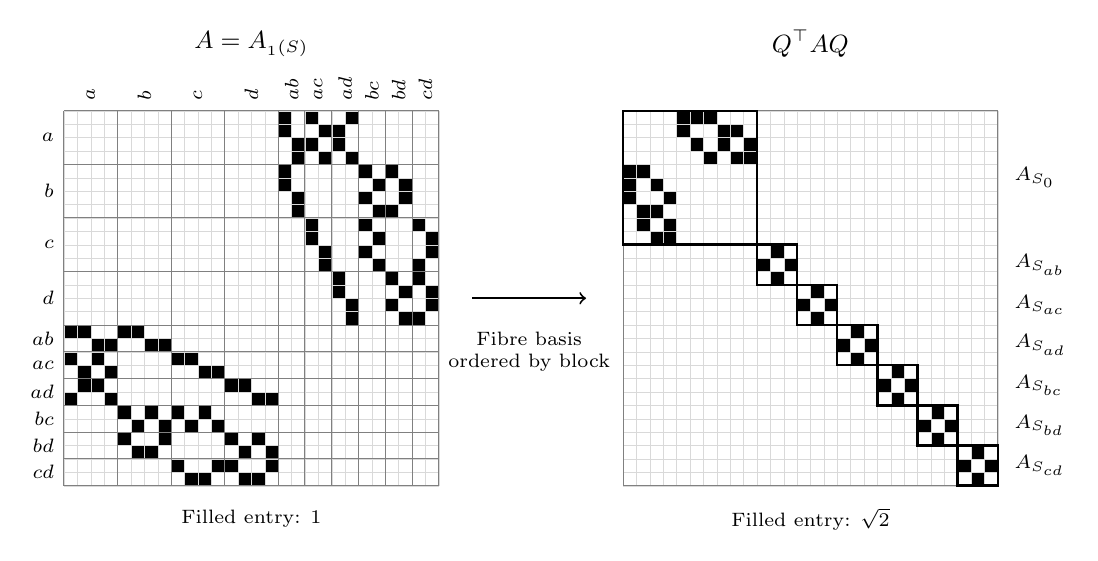
\begin{tikzpicture}[
  x=.17cm,y=-.17cm,
  entry/.style={fill=black},
  gridline/.style={draw=black!15,line width=.1pt},
  fibreline/.style={draw=black!50,line width=.35pt},
  block/.style={draw=black,line width=.9pt},
  every node/.style={font=\scriptsize,inner sep=1pt},
]
\node[font=\small] at (14,-5) {$A=A_{\CFI_1(S)}$};
\foreach \v/\e/\k in {
  0/0/0,0/1/1,0/2/2,
  1/0/0,1/3/1,1/4/2,
  2/1/0,2/3/1,2/5/2,
  3/2/0,3/4/1,3/5/2
} {
  \ifnum\v=0
    \def\fibrebits{0/0/0/1,1/0/1/0,2/1/0/0,3/1/1/1}
  \else
    \def\fibrebits{0/0/0/0,1/0/1/1,2/1/0/1,3/1/1/0}
  \fi
  \foreach \r/\first/\second/\third in \fibrebits {
    \ifcase\k\edef\bit{\first}\or\edef\bit{\second}\or\edef\bit{\third}\fi
    \pgfmathtruncatemacro{\row}{4*\v+\r}
    \pgfmathtruncatemacro{\col}{16+2*\e+\bit}
    \fill[entry] (\col,\row) rectangle ++(1,1);
    \fill[entry] (\row,\col) rectangle ++(1,1);
  }
}
\foreach \position in {0,...,28} {
  \draw[gridline] (\position,0)--(\position,28);
  \draw[gridline] (0,\position)--(28,\position);
}
\foreach \boundary in {0,4,8,12,16,18,20,22,24,26,28} {
  \draw[fibreline] (\boundary,0)--(\boundary,28);
  \draw[fibreline] (0,\boundary)--(28,\boundary);
}
\foreach \position/\name in {
  2/a,6/b,10/c,14/d,17/ab,19/ac,21/ad,23/bc,25/bd,27/cd
} {
  \node[anchor=west,rotate=90] at (\position,-.5) {$\name$};
  \node[anchor=east] at (-.5,\position) {$\name$};
}
\node at (14,30.5) {Filled entry: $1$};

\draw[->,line width=.7pt] (30.5,14)--(39,14);
\node[align=center] at (34.75,18) {Fibre basis\\ordered by block};

\begin{scope}[xshift=7.1cm]
  \node[font=\small] at (14,-5) {$Q^{\top}AQ$};
  \foreach \e/\u/\v in {0/0/1,1/0/2,2/0/3,3/1/2,4/1/3,5/2/3} {
    \pgfmathtruncatemacro{\subdivision}{4+\e}
    \foreach \endpoint in {\u,\v} {
      \fill[entry] (\subdivision,\endpoint) rectangle ++(1,1);
      \fill[entry] (\endpoint,\subdivision) rectangle ++(1,1);
    }
    \pgfmathtruncatemacro{\start}{10+3*\e}
    \foreach \r/\c in {0/1,1/0,1/2,2/1} {
      \fill[entry] ({\start+\c},{\start+\r}) rectangle ++(1,1);
    }
  }
  \foreach \position in {0,...,28} {
    \draw[gridline] (\position,0)--(\position,28);
    \draw[gridline] (0,\position)--(28,\position);
  }
  \draw[fibreline] (0,0) rectangle (28,28);
  \draw[block] (0,0) rectangle (10,10);
  \node[anchor=west] at (29,5) {$A_{S_0}$};
  \foreach \j/\e in {0/ab,1/ac,2/ad,3/bc,4/bd,5/cd} {
    \pgfmathtruncatemacro{\start}{10+3*\j}
    \draw[block] (\start,\start) rectangle ++(3,3);
    \node[anchor=west] at (29,{\start+1.5}) {$A_{S_{\e}}$};
  }
  \node at (14,30.5) {Filled entry: $\sqrt2$};
\end{scope}
\end{tikzpicture}
\caption{Block decomposition for the subdivision $S$ of $\Gamma=K_4$
on vertices $a,b,c,d$, with tree attachments omitted.
The left matrix groups the $28$ CFI vertices by fibre and uses odd parity
at $a$. Within fibres, the bit vectors are in lexicographic order,
with incident-edge coordinates ordered by their labels.
The columns of $Q$ are the fibre basis vectors from the proof, ordered
first by the ten constant directions and then by the three sign directions
over $v,e,w$ for each edge $e=vw$ of $K_4$.
The right matrix has one $10\times10$ block $A_{S_0}=\sqrt2 A_S$ and
six $3\times3$ blocks $A_{S_e}$; unfilled entries are zero.
Both CFI parities give the same right matrix.}
\label{fig:ss-cfi-blocks}
\end{figure}


Combining these root-coordinate matrices with the tree blocks in
\cref{eq:ss-tree-blocks} shows that the subspaces $U_0$ and $U_e$
are invariant and that the adjacency matrix of $\widehat{\CFI}_i(S)$ has the block diagonal form
\cref{eq:ss-rooted-blocks} in the stated bases.
\end{proof}

\begin{lemma}\label{lem:ss-cfi-spectrum}
Let $\Gamma$ be a connected cubic graph, and let $S$ be its subdivision
with one new vertex on each edge.
There is a family $(T_z)_{z\in V(S)}$ of trees in $\mathcal T$ such that the
CFI-compatible rooted products $\widehat{\CFI}_0(S)$ and $\widehat{\CFI}_1(S)$
are non-isomorphic, bipartite, cospectral, nonsingular graphs with
simple spectrum and maximum degree at most six.
\end{lemma}
\begin{proof}
Since the isomorphism type of $\CFI_1(S)$ is independent of the
distinguished vertex $v_*$, we choose $v_*\in V(\Gamma)$.
Let $S_0$ and $S_e$ be the weighted graphs from \cref{lem:ss-cfi-blocks}.
We apply \cref{lem:ss-separation} to these graphs,
with $Z=V(S)$.
They are connected and have nonzero edge weights. Their vertex sets
$V(S)$ and $\{v,e,w\}$ for $e=vw\in E(\Gamma)$ are pairwise distinct.
By that lemma, there is one tree $T_z\in\mathcal T$ for each
$z\in V(S)$ such that the rooted products $\widehat S_0$ and
$\widehat S_e$ are nonsingular and have simple, pairwise disjoint
spectra.
The block matrix in \cref{eq:ss-rooted-blocks} therefore has simple
spectrum and is nonsingular.
By \cref{lem:ss-cfi-blocks}, the adjacency matrices of
$\widehat{\CFI}_0(S)$ and $\widehat{\CFI}_1(S)$ are both
orthogonally similar to this matrix, so the two rooted products are
cospectral, nonsingular and have simple spectrum.

The graphs $\widehat{\CFI}_0(S)$ and $\widehat{\CFI}_1(S)$ are
non-isomorphic because their maximal subgraphs of minimum degree at least two
are the non-isomorphic graphs $\CFI_0(S)$ and $\CFI_1(S)$.
Both rooted products are bipartite, since each CFI graph is bipartite
and attaching trees preserves bipartiteness.
The CFI graphs have maximum degree four, and each attached tree is
subcubic with root degree at most two, so the rooted products have
maximum degree at most six.
\end{proof}

\begin{proof}[Proof of \cref{lem:ss-transfer}]
\Cref{lem:ss-cfi-spectrum} needs the subdivision of a connected cubic
graph as its base, so we first replace $B$ by such a base $S$ that
contains $B$ as a minor.
Let $t$ be an integer with $t\geq\max\{4,|V(B)|\}$, so that $B$ is a minor of $K_t$ and the
cycles below have length at least three.
Let $\Gamma$ be the connected cubic graph obtained from $K_t$ by
replacing each vertex with a cycle of length $t-1$ and attaching its
$t-1$ incident edges to distinct cycle vertices.
Let $S$ be the
subdivision of $\Gamma$ with one new vertex on each edge.
Contracting one edge at each subdivision vertex of $S$ gives $\Gamma$,
and contracting the replacement cycles of $\Gamma$ gives $K_t$, so $B$
is a minor of $S$.
Hence $\CFI_0(S)\equiv_{\mathcal C}\CFI_1(S)$ follows from the
assumption $\CFI_0(B)\equiv_{\mathcal C}\CFI_1(B)$ by
\cite[Corollary~5.7]{Roberson2026}.
Using the trees from \cref{lem:ss-cfi-spectrum}, let
$G=\widehat{\CFI}_0(S)$ and $G'=\widehat{\CFI}_1(S)$.
That lemma shows that $G$ and $G'$ are non-isomorphic, bipartite,
cospectral and nonsingular, with simple spectrum and maximum degree at
most six. By \cref{lem:ss-attachments}, $G\equiv_{\mathcal C}G'$.
\end{proof}

\begin{remark}\label{rem:ss-minor-necessity}
For the families in \cref{prop:closure}, arbitrarily large clique minors
suffice for completeness.
It is natural to ask whether every class complete on simple
spectrum must contain graphs with arbitrarily large clique minors.
The weak Roberson conjecture states that for every proper minor-closed
graph class $\mathcal C$ there are non-isomorphic graphs
$G\equiv_{\mathcal C}G'$~\cite[Conjecture~5 and Theorem~8.4]{Roberson2026}.
An affirmative answer to the question above implies this conjecture,
because a proper minor-closed class $\mathcal C$ excludes some $K_t$,
so, under an affirmative answer, there are non-isomorphic graphs
$G\equiv_{\mathcal C}G'$ with simple spectrum.
By \cref{lem:ss-transfer}, non-isomorphic graphs
$G\equiv_{\mathcal C}G'$ with simple spectrum exist for every
minor-closed class $\mathcal C$ that
admits a connected graph $B$ with $\CFI_0(B)\equiv_{\mathcal C}\CFI_1(B)$.
\end{remark}
